\documentclass[a4paper, 12pt]{article}
\usepackage[french]{babel}
\usepackage[utf8]{inputenc}
\usepackage[T1]{fontenc}
\usepackage{fancyvrb}
\usepackage{graphicx}
\usepackage{geometry}
\usepackage{tabularx}
\usepackage{caption}
\usepackage{amsmath}
%\usepackage{listings}
%\usepackage[usenames,dvipsnames,svgnames,table]{xcolor}
%\usepackage{pdfpages}
\usepackage[backend=bibtex]{biblatex}
\addbibresource{biblio.bib}
\geometry{hmargin=2.5cm,vmargin=2.5cm}

% Title Page
\begin{document}
\begin{titlepage}
\newcommand{\HRule}{\rule{\linewidth}{0.5mm}}

\begin{center}

\HRule \\[0.4cm]
{ \huge Projet de datamining}\\[0.4cm]
\HRule \\[2cm]

\vspace{2cm}

Chloé Gobé \\
Venceslas Danguy des Déserts \\ 
Eymard Houdeville


\vspace{2cm}


\end{center}
\end{titlepage}

%\maketitle
%\newpage

\tableofcontents
\newpage

\section*{Introduction}
\addcontentsline{toc}{section}{Introduction}

Ce projet a été réalisé dans le cadre du cours IS3024, \textit{Des données à la connaissance}. Nous avions pour objectif de prédire le taux de remboursement d'un médicament en fonction d'autres données telles que le prix, les avis des différentes commissions, le laboratoire de production, etc. 

\section{Ensemble de données}

Nous nous sommes basés sur la Base de Données Publique et officielle des Médicaments \cite{database} (BDPM). \\

Voici le schéma complet de cette base de données :

\begin{center}
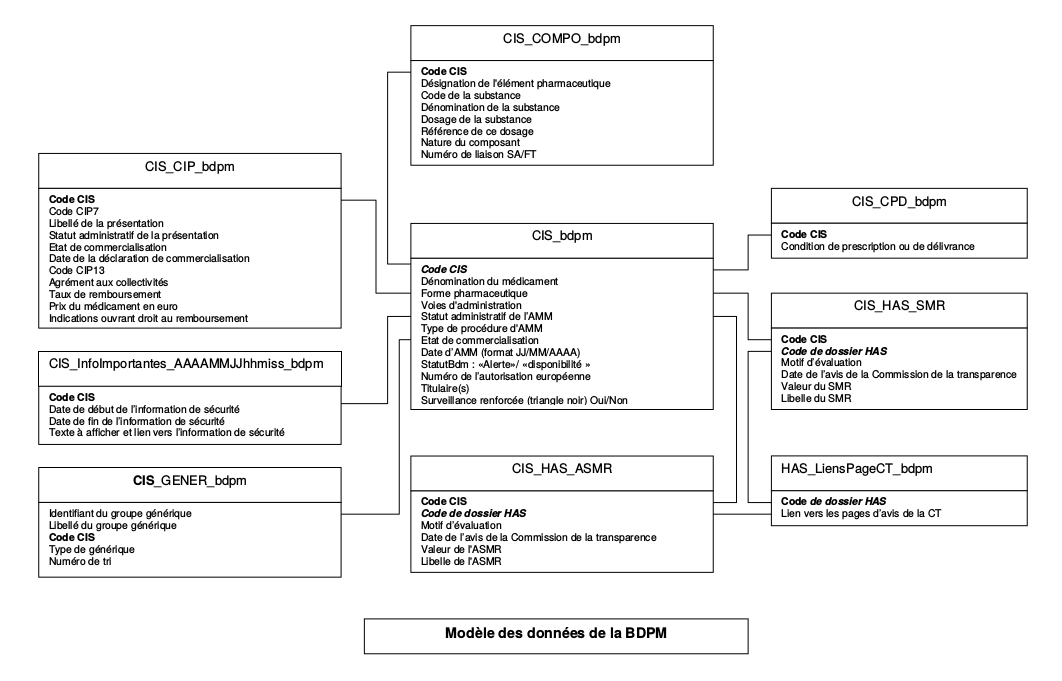
\includegraphics[scale=0.45]{pics/schema.png}
\captionof{figure}{Schéma de la base de données}
\end{center} 

Il est possible de récupérer un dump récent de cette base de données sur le site \textit{www.data.gouv.fr}.

\smallskip

Les tables les plus importantes sont les suivantes :
\begin{description}
\item[CIS\_bdpm : ] Contient une ligne par médicament avec son nom, son identifiant unique (code CIS), sa forme pharmaceutique, ses voies d'administration, ainsi que des informations sur les différentes procédures et status.
\item[CIS\_CIP\_bdpm :] Cette table contient une ligne par présentation, une présentation étant en quelque sorte une instance d'un médicament. Par exemple le médicament \textit{Doliprane en comprimés} peut être vendu par boîte de 8 ou 16 comprimés, et à une concentration de 500 mg ou 1000 mg. Ce sont ces présentations qui ont un prix et un taux de remboursement fixés par les différentes commissions. 
\item[CIS\_HAS\_SMR et CIS\_HAS\_ASMR :] Contiennent les avis des commissions sur le \textit{Service Médical Rendu} (SMR, l'utilité du médicament pour une pathologie donnée), ainsi que sur l'\textit{Amélioration du Service Médical Rendu} (ASMR, utilité du médicament pour une pathologie donnée par rapport aux traitements pré-existants). La commission rend un avis pour chaque pathologie pour laquelle le médicament peut avoir un intérêt, ainsi un médicament peut-il avoir un SMR bon pour une pathologie et mauvais pour une autre.
\end{description}

\smallskip

La base de données contient aussi des informations sur l'existence ou non de génériques, ainsi que sur la présence d'informations "de sécurité", mais nous avons choisi de ne pas les inclure pour garder un modèle simple. Il doit toutefois être possible d'améliorer nos résultats en les utilisant (la présence d'un générique doit par exemple fortement influencer le taux de remboursement du médicament original).

\section{Nettoyage des données}

Bien que cette base de donnée soit officielle, la qualité des données laisse à désirer. Nous avons donc du remanier une bonne partie des champs pour proprifier les données.

\subsection{Médicaments - CIS\_bdpm}

\subsubsection*{Formes galléniques}

Les formes galléniques sont très nombreuses : le dataset en compte au départ 401 différentes. En regardant le champ de près, on s'aperçoit que sont distingués par exemple les \textit{comprimés}, les \textit{comprimés sécables} ou les \textit{comprimés enrobés}. Il y a aussi des erreurs d'écriture, ainsi l'un des médicaments a-t-il pour forme gallénique \textit{capsule molle ou} (littéralement). Nous avons estimé que nous n'avions pas besoin d'un tel niveau de détail et avons donc fusionné les différentes formes de façon à n'en garder que 67. L'idée est de générale est de mettre ensemble tous les comprimés, toutes les pommades, etc, et de regarder "à la main" les formes restantes pour vérifier qu'il ne reste pas d'aberration ou de formes pouvant être fusionnée.

\subsubsection*{Utilisation de types "catégories"}

Pandas possède un type \textit{category} utilisé pour représenter un champ correspondant à une unique catégorie parmis plusieurs. L'utilisation de ce type de données ne change pas le contenu de la cellule en soi mais facilite le traitement ultérieur pour calculer des statistiques ou transformer l'entrée de façon à pouvoir la donner à un modèle d'apprentissage. Nous avons donc taggés comme étant des catégories les champs suivants : 
\begin{itemize}
\item galenic\_form
\item route\_of\_administration
\item owners
\item commercialisation\_status
\item clearance\_status
\item clearance\_type
\item bdm\_status
\item enhanced\_monitoring
\end{itemize}

\subsubsection*{Voies d'administration}

Les différentes voies d'administration utilisables pour un médicament donné sont présentées dans le dataset comme une liste d'éléments séparés par des point-virgules. 

Exemple : \textit{infiltration;intra-articulaire;périarticulaire;péridurale;périneurale}

Cette liste n'est pas utilisable par pandas en l'état, nous l'avons donc transformée en un vecteur de longueur l'ensemble des voies possibles, et de valeur 1 si la voie est applicable, 0 sinon.

%TODO : Utiliser différentes colonnes ?

\subsubsection*{Dates}

Il faut enfin parser tous les champs contenant des dates de façon à ce que pandas les reconnaisse comme tel et non plus comme des chaînes de charactères. Cela permet d'établir une relation d'ordre (temporelle) entre différentes valeurs.

\subsection{Présentations - CIS\_CIP\_bdpm}

En plus des traitements sur les dates et les types catégories que nous appliquons aussi, il y a quelques champs spécifiques à traiter.

\subsubsection*{Prix}

Nous avons décidé de supprimer tous les médicaments n'ayant pas de prix de vente. Après vérification nous sommes arrivés à la conclusion qu'une absence de prix (qui va de pair avec une absence de taux de remboursement) dans la base de donnée signifie simplement que le médicament n'est pas remboursé par la Sécurité Sociale. Nous avons choisi de ne pas inclure ces médicaments dans notre ensemble de données, mais il aurait pu être intéressant de tenter de prédire aussi un taux de 0\%.

\subsubsection*{Taux de remboursements}

Nous nous sommes que s'il existe peu de taux différents (15\%, 30\%, 65\% et 100\%), ces taux pouvaient être écrits dans deux formats différents dans la base : avec et sans espace entre le dernier chiffre et le \%. Ainsi trouve-t-on des médicaments remboursés à \textit{15\%} et d'autres à \textit{15 \%}. Nous avons donc enlevé les espaces partout...

\subsection{SMR et ASMR - CIS\_HAS\_ASMR\_bdpm, CIS\_HAS\_SMR\_bdpm}

Les avis SMR et ASMR sont fixés par des commissions et rendent compte du service rendu ou de son amélioration \cite{smrasmr}. Ils sont normalement déterminants dans le choix du taux de remboursement \cite{fixation}. Les laboratoires déposent une requête d'évaluation pour un médicament donné et pour un ensemble d'indications thérapeuthiques. Les commissions rendent ensuite un avis pour chacune de ces indications. La base de données ne contient malheureusement que les avis rendus après 2002... Comme il est compliqué d'analyser les commentaires textuels de la commission, nous avons choisi de ne garder que les notes qui vont de un à cinq. Un médicament donné à donc plusieurs notes : une par indication thérapeutique. Afin de simplifier le modèle, nous avons regroupés ces notes en fonction de leurs valeurs et les avons comptées. Ainsi, dans notre dataset final, les notes d'un médicament se présentent comme suit :
\begin{description}
\item[SMR - insuffisant :] un avis
\item[SMR - faible :] zéro avis
\item[SMR - modéré :] zéro avis
\item[SMR - important :] deux avis
\item[SMR - majeur :] zéro avis
\end{description}
Ce médicament rend donc un service médical insuffisant pour l'une des indications évaluées, mais important pour les deux autres.
\section{Modèles et entraînements}

\section*{Conclusion}
\addcontentsline{toc}{section}{Conclusion}

\printbibliography
\end{document}